\chapter{Spatial Explanations using Hierarchical Intervention}
\label{chp:proposed}
\label{sec:hei_intervention}

\section{Introduction}
Hierarchical Intervention is an extension of the intervention approach. The idea behind hierarchical intervention is to improve our explanations by grouping together spatially colocated polygons in our candidate explanation. We divide the space into a set of levels. The first level contains the entire space as one cluster, while the last level contains each zone or each point in each cluster.

\section{Spatial Partitioning/Clustering}
There are several approaches to cluster data. Each clustering approach has a large impact on the resulting explanations. In order to understand the issues with explanations using spatial clustering, we need to have an understanding of the clustering approaches.

\subsection{R-Tree}
An R-Tree is a data structure which is commonly used for spatial data indexing. The idea behind the R-Tree is similar to the idea behind a binary tree i.e. It is faster to query data if it is stored in the form of a hierarchy\citep{guttman1984r}. In an R Tree, this hierarchy exists in the form of Minimum Bounding Rectangles(MBR).

\begin{figure}[ht]
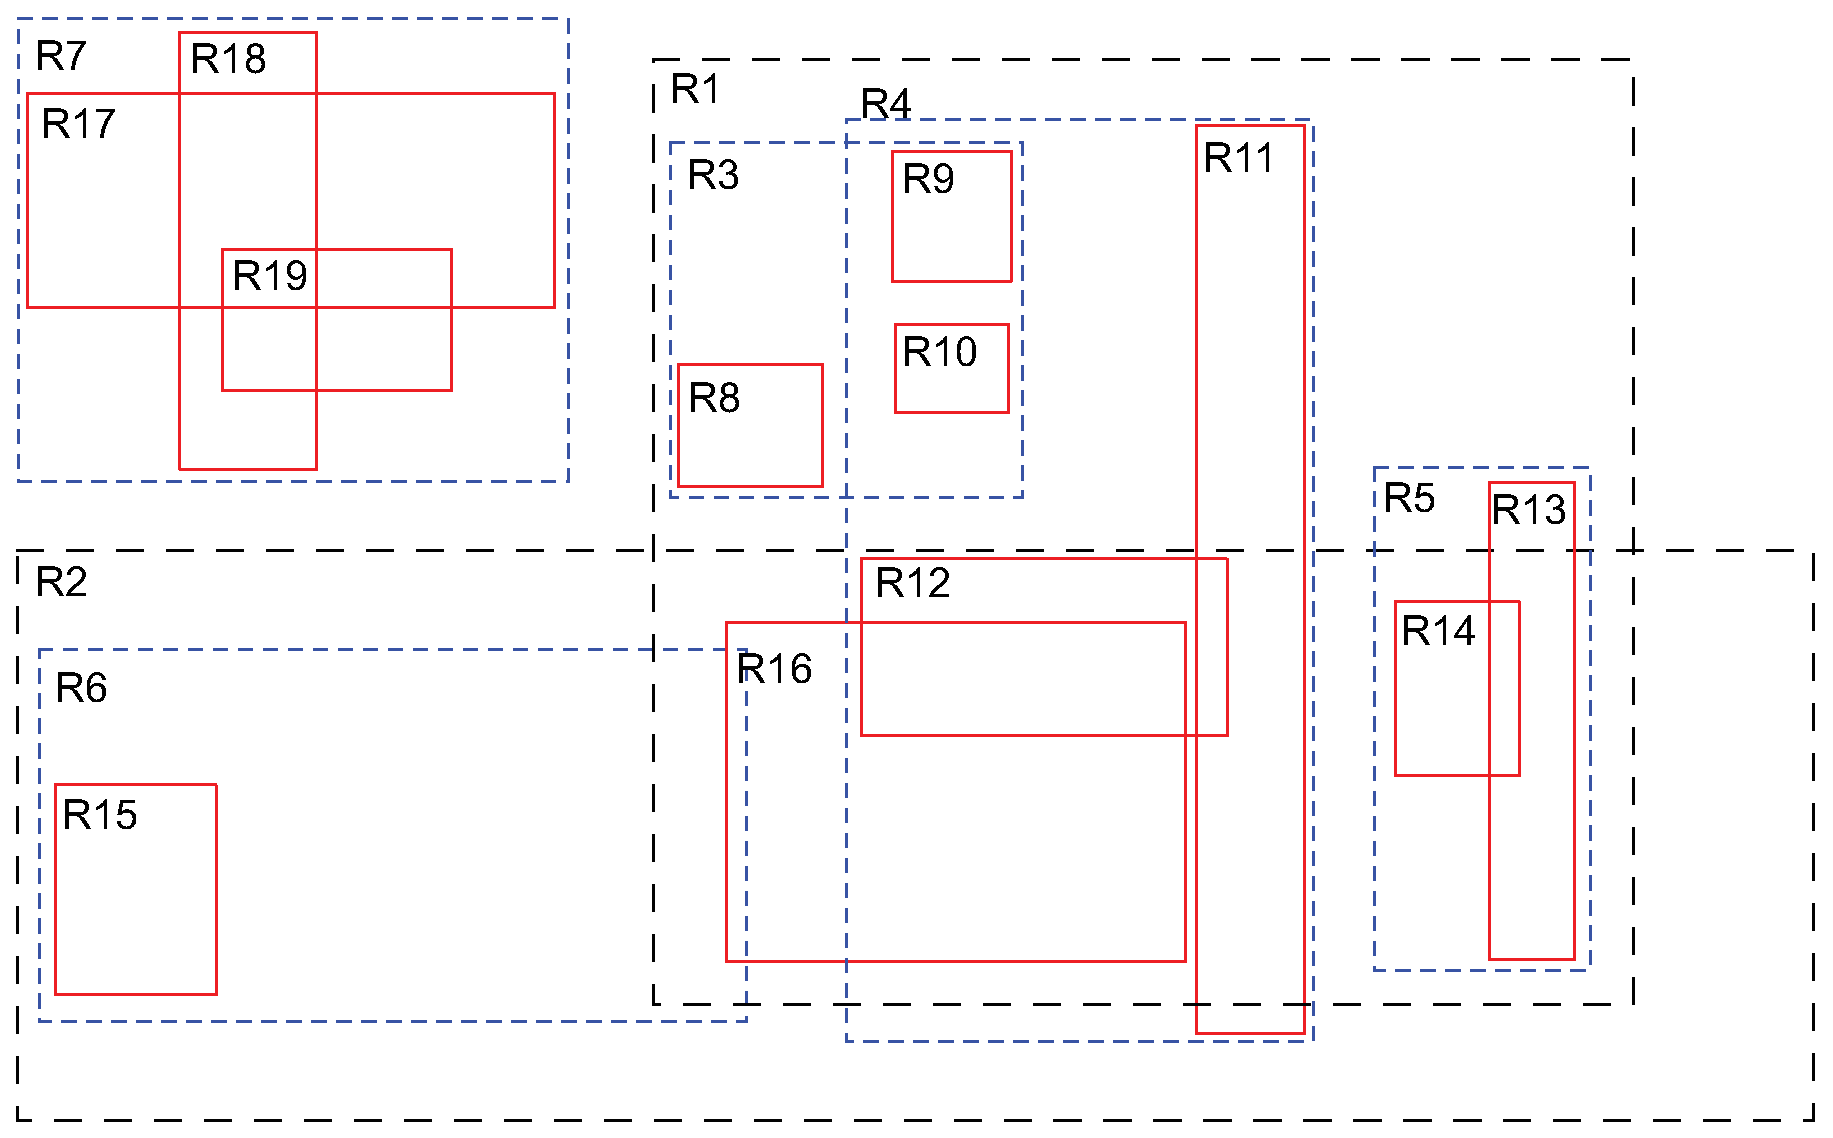
\includegraphics[width=\columnwidth]{rtree}
\caption{An illustration of R-Tree}
\label{fig:rtree}
\end{figure}

The top level of an R Tree consists of a set of MBRs which cover a large spatial area. Each MBR can now be subdivided into further MBRs which makes up the second level of the tree and so forth. At the leaf nodes of the tree, each node consists of a single object in our underlying data.

There are three main considerations when building an R Tree: insertion, deletion, and search. In order to insert data, it is important to consider that the tree is balanced. A balanced tree results in faster search since the depth of the tree is reduced. The same thing needs to be taken into consideration with deletion.
In order to insert an element, a heuristic is usually involved. The main objective when inserting into an R-Tree is to minimize the splitting and enlargement. If an element can be inserted into an existing MBR, then it is preferred. Otherwise, existing MBR's are either split or enlarged.

When elements from an R-Tree are deleted, the parent nodes are also taken into consideration. This is because deleting elements may result in a change in the parent MBR as well, unlike a B-Tree. B-Tree is an indexing structure inspired from a binary tree \citep{bayer1970organization}. An R-Tree maintains a minimum utilization constant into consideration when deleting. If a node in the R-Tree is below the minimum utilization, the elements are reinserted.

Finally, the main purpose of constructing an R-Tree is to optimize search speed. If the branching factor of the R-Tree is $\lambda$ and there are $n$ elements that are indexed, then the search cost of the R-Tree is $\log_{\lambda}{n}$ assuming that the tree is balanced.


\subsection{R*-Tree}
R* Tree is a variation of R-Tree\citep{beckmann1990r}. The objective of an R*-Tree is to minimize overlaps and coverage in an R-Tree. It also optimizes for margin and area. The idea behind R*-Tree which helps in achieving its objective is to use the perimeter of the MBR as a heuristic when splitting and creating R-Trees.

Unlike R-Trees, the insert operation of an R* Tree also incorporates deletion. When an element is added to an R-Tree, an existing MBR is either extended or split. However, ordering of the insertion in an R-Tree deforms existing MBRs and may lead to more coverage. The R* Tree solves this problem by removing elements from nodes and reinserting them. Splitting of MBRs is also based on perimeter. There are multiple ways to split an MBR, but if its split based on the least resulting perimeter as a heuristic, then this heuristic leads to better partitioning with less overlaps.

The search and delete operations of an R* Tree are the same as an R Tree.

\subsection{K-means clustering/Voronoi partitioning}
K means clustering is an algorithm designed to cluster a group of points \citep{macqueen1967some}. As the name suggests, the user decides the number of clusters that he/she wants. $K$ represents the number of clusters. The algorithm randomly selects $k$ seed points. The seed points can also be selected using a heuristic to improve the clustering. The points closest to each of the seed points form clusters. The k means algorithm is iterative. Which means it does not end there. The centroids of the clusters are used as new seed points and the process is repeated until the centroids are constant. Algorithm~\ref{alg:kmeans} shows our version of the kmeans algorithm where the selectivity is used as a metric for judging the clusters.

% TODO Add reference to greedy hierarchical clustering
% Let $D$ be our spatial dataset. Let $P$ be a set of distinct polygons over our dataset $D$. We define a set of distinct clusters of polygons $P_h$. The polygons can be clustered in many different ways but we used greedy hierarchical clustering because of its speed and relevance to the problem. Let $C$ be the set of centroids in $P$ i.e. $\forall p_i \in P$, $c_i$ is the centroid for $p_i$, where $c_i \in C$. We define a set of $n$ levels, $L = \{l_1, l_2,...,l_n\}$. We represent each centroid in $C$ on a cartesian plane where $x_i$ is the first dimension of the centroid $c_i$ and $y_i$ is the second dimension of the centroid $c_i$. Let $x_{min}$, $x_{max}$ be the minimum and maximum value for $x_i$ respectively. Let $y_{min}$, $y_{max}$ be the minimum and maximum values of $y_i$ respectively. There is a radius associated with each level in $L$. Let $r_i$ be the radius for level $l_i$ in $L$, We can define $r_i$ in general as,
% $$r_i = \frac{\sqrt{(y_{max}-y_{min})^2+(x_{max}-x_{min})^2}}{2^{i-1}}$$

% The set of clusters,$G_i$, for level $l_i$ can be defined as $G_i=\{p_k|(x_k^2 + y_k^2 < r_i^2)\}\forall p_k \in P$. Any possible set cover of $P$ in $G_i$ can now be considered for inclusion in $P_h$. One implementation of this approach is covered in Section~\ref{sec:hie_impl}


\subsection{Hierarchical Greedy Clustering}
Hierarchical Greedy Clustering is a popular algorithm in data visualizations because of its speed \citep{hgclustering}. The idea behind this algorithm is to randomly select points and create clusters around them.

Let $D$ be our spatial dataset. Let $P$ be a set of distinct polygons over our dataset $D$. We define a set of distinct clusters of polygons $P_h$. Let $C$ be the set of centroids in $P$ i.e. $\forall p_i \in P$, $c_i$ is the centroid for $p_i$, where $c_i \in C$. We define a set of $n$ levels, $L = \{l_1, l_2,...,l_n\}$. We represent each centroid in $C$ on a Cartesian plane where $x_i$ is the first dimension of the centroid $c_i$ and $y_i$ is the second dimension of the centroid $c_i$. Let $x_{min}$, $x_{max}$ be the minimum and maximum value for $x_i$ respectively. Let $y_{min}$, $y_{max}$ be the minimum and maximum values of $y_i$ respectively. There is a radius associated with each level in $L$. Let $r_i$ be the radius for level $l_i$ in $L$, We can define $r_i$ in general as,
$$r_i = \frac{\sqrt{(y_{max}-y_{min})^2+(x_{max}-x_{min})^2}}{2^{i-1}}$$

The set of clusters,$G_i$, for level $l_i$ can be defined as $G_i=\{p_k|(x_k^2 + y_k^2 < r_i^2)\}\forall p_k \in P$. The algorithm for the implementation of this approach is covered in Section~\ref{sec:hie_impl}.

Greedy Hierarchical Clustering turned out to have a drawback when we use it for explanations. It selects seed points randomly. This means that in each level, the clusters can be highly imbalanced. We compared this approach to K means(Voronoi partitioning)\citep{hartigan1979algorithm,aurenhammer2000voronoi}, R Tree\citep{guttman1984r} and R* Tree\citep{beckmann1990r}.

The main idea behind the hierarchical intervention approach, regardless of the partitioning algorithm, is to help us in increasing the domain for our degree of explanation. Since intervention is a subset of this approach, the domain is at least as large as that for intervention.


\section{Extending Hierarchical Intervention}
\label{sec:extending_hi}

In order to get the most out of Hierarchical Intervention, we introduce two new metrics: Intensity and Influence.

\subsection{Intensity}
\label{sec:intensity}

%What is relevance
We define intensity as a metric which measures the standalone value of the explanation. The relevance metric borrows a lot from our definition of aggravation. It might be convenient to think of a web search engine when we are looking at the intensity metric. When we use a search engine, we provide a search term as a query. The search engine looks at all the pages in its database and returns the results in order of relevance. The top results in the search engine may not have a significant effect on the entire web if they were to be removed. However, the top result in the search engine has the highest relation to the data. For example, the top result for a search engine which uses tf-idf might be a page containing the highest frequency of the search term\citep{robertson2004understanding}.

%Formal definition of relevance
Let $D$ be our dataset. Let $\phi$ be our candidate explanation. Let $R$ be the function which maps our dataset to the value of our observation. Then we can define intensity as,
$$intensity = |R(\sigma (D)) - R(\sigma_\phi (D))|$$

\subsection{Influence}
\label{sec:influence}
% What is influence
We define influence as a metric which measures the value of the explanation compared to the entire dataset. The influence metric borrows from our definition of intervention. The influence metric measures how much the observation would be affected if we remove the data related to our explanation(the \textit{influence} of our explanation on the observation). We can use the analogy of the search engine again here. One of the earliest algorithms used by Google to rank webpages used links to other pages\citep{brin1998anatomy}. The page which was linked the most on a variety of websites was ranked higher. If you remove a highly relevant page, many other pages might not exist. Influence uses the same principle.

%Formal definition of influence
Let $D$ be our dataset. Let $\phi$ be our candidate explanation. Let $R$ be the function which maps our dataset to the value of our observation. Then we can define relevance as,
$$influence = |R(\sigma(D)) - R(\sigma_{\neg \phi} (D)) |$$

The greater the value of influence, the more its impact on the observation.

Our evaluation metrics suggest that influence and intensity explain data in different ways. Explanations with higher influence tend to give predicates which cover a larger area while explanations with higher intensity tend to give predicates which cover a small area. We can balance out these two metrics according to the preferences of the observer. We define the \textit{explanation index}, $\epsilon$ as:
$$\epsilon = \alpha \times influence + (1-\alpha) \times intensity$$
$\alpha$ is the \textit{explanation coefficient}. It is a variable whose value is decided by the user.

Explanations given by Hierarchical Intervention can be ranked on the basis of the explanation index.


\section{Implementation}
\label{sec:implementation}
We created an implementation of the our system as a proof of concept. Our system uses a web based GUI for visualization while the backend processing is done using Spark\citep{shanahan2015large}. Fig.~\ref{fig:framework} shows the archicture diagram of the entiresystem. We borrowed from the MapReduce implementation of Salient Features from the Data Polygamy Framework\citep{chirigati2016data}. There are three main stages in our system pipeline: Preprocessing, User Input, and Explanation Visualization. The preprocessing stage is different for each approach to explanation. The user input stage can be divided into two further parts: The user observation, and the type of explanation the user is interested in. An example of the explanation approach would be intervention. The user observation can be one of the attributes the user wants to observe e.g. a mathematical expression spanning several aggregate queries.


\label{aggravation_impl}
The aggravation approach that we use makes several optimizations to the naive approach one may come up with. A naive approach may consider each candidate explanation and calculate the degree of explanation by aggravation for each one. However, using such an approach would take a long time. If the attribute which we are looking into for explanation has $m$ possible values, it would take $O(m)$ queries to come up with top explanations. If we have $r$ rows in our dataset and each observation query has a linear time complexity, our total time complexity would be $O(rm)$. We can reduce the time complexity by a large factor if we make each candidate explanation cover a larger range of the dataset.

%Talk about bucketing
As mentioned in Section~\ref{sec:aggravation}, we use bucketing to reduce the number of permutations. We use the standard deviation, $\sigma$, of each attribute to separate values which are near the average from the others. We can get the minimum and standard deviation of each attribute over a single iteration of our table in $O(r)$ time. Since the bucket for each value of the attribute can be calculated in constant time, we create a new table containing the bucket value of the attribute in $O(r)$ time.

%Talk about grouping
Since we bucketed our data, the number of candidate explanations have been reduced to $O(\big(\frac{m}{\sigma}\big))$. However, there is still room for improvement. Our observation is always an aggregate query. If we group on the explanation attributes, we can still get all of the corresponding values of the observation in one iteration of the data, making our time complexity $O(r)$.

%Talk about zoning
Another component of our system is spatial data. Our system is designed to handle spatial observations and explanations. When given a spatial observation, our system filters out the data with the spatial predicate given in the observation. The remaining data is used just like any other explanation task. Spatial Explanations, on the other hand, require a bit more work. Given a set of polygons, doing a spatial join with the data is a very expensive process. Our system performs a spatial join once and assigns each tuple an ID based on which polygon it belongs to. The ID can now be used like a regular attribute for explanation.


\label{intervention_impl}

%Talk about grouping
Intervention is another approach that our system uses. Some of the work we did to optimize aggravation cannot be used to improve the time complexity for intervention. This is because intervention looks at the effect of removing data. While we could use a single iteration of the data for aggravation. We cannot do so for intervention because removing one portion of the data completely changes what the observation looks like. We can still use bucketing to reduce the number of combinations.


\subsection{Hierarchical Intervention}
\label{sec:hie_impl}
Hierarchical intervention is an improvement on top of the intervention approach. The main idea behind hierarchical intervention is to group spatially colocated points/polygons together in an attempt to improve explanations. We use a partitioning algorithm to create clusters. The base case of our algorithm consists of clusters with a single node each. This makes the results of intervention a subset of the results of hierarchical clustering. Algorithm~\ref{alg:hie} highlights the algorithm that we used for our implementation of greedy hierarchical clustering. Note that each level in the hierarchy is a set cover of all the nodes.

Greedy Hierarchical Clustering is an iterative algorithm. The base case(Algorithm.~\ref{alg:hie};line 27) is when we reach the lowest level in the hierarchy where we have individual points or zones. We start off with the highest level in the hierarchy(Algorithm.~\ref{alg:hie};line 4). We select random points and form clusters around them(Algorithm.~\ref{alg:hie};line 16). In the following iteration we reduce the size of the cluster by a constant factor(Algorithm.~\ref{alg:hie};line 8) and repeat until we reach the base case.


% Talk about clustering
\begin{algorithm}
\caption{Algorithm for Hierarchical clustering}\label{alg:hie}
\begin{algorithmic}[1]
\Procedure{Cluster}{$max\_radius,points$}
  	\State $input: max\_radius, points$
      \State $output: hierarchy\_of\_clusters$
   	\State $level \gets 0$

  	\State $isBaseCase \gets false$
  	\While{isBaseCase = false}
  	    \State $level \gets level + 1$
  	    \State $levelRadius \gets \frac{max\_radius}{2.0^{level}}$

  	 	\State $hierarchy \gets \emptyset$

  	    \State $unusedPoints \gets \emptyset$

      	\For{$point \gets points$}
      		\State $unusedPoints \gets unusedPoint \cup point$
      	\EndFor

      	\While{$unusedPoints.size > 0$}
  			\State $cluster \gets \emptyset$

  			\State {$centroid \gets $random point from points}

  			\For{$point \gets unusedPoints$}
  				\If{point inside levelRadius}
  					\State $cluster \gets cluster \cup point$
  					\State $unusedPoint \gets unusedPoints - point$
                 \EndIf
  			\EndFor

  			\State $hierarchy \gets hierarchy \cup cluster$

      	\EndWhile
        \algstore{myalg}
    \end{algorithmic}
    \end{algorithm}
    \begin{algorithm}
    \begin{algorithmic} [1]
    \algrestore{myalg}
      	\State $hierarchy\_of\_clusters \gets hierarchy\_of\_clusters \cup \{level,hierarchy\}$

      	\State $isBaseCase \gets true$

  		\For{$cluster \gets heirarchy$}
  			\If {$cluster.size > 1$}
  				\State $isBaseCase \gets false$
  			\EndIf
  		\EndFor
  	\EndWhile
  	\State \textbf{return} $hierarchy\_of\_clusters$

\EndProcedure
\end{algorithmic}
\end{algorithm}

\begin{figure}
%   \begin{algorithmic}[1]
%   % 	\State $input: max_radius, points$
%   %     \State $output: hierarchy_of_clusters$
%   %  	\State $level \gets 0$

%   % 	\State $isBaseCase \gets false$
%   % 	\While{isBaseCase = false}
%   % 	    \State $level \gets level + 1$
%   % 	    \State $levelRadius \gets \frac{max_radius}{2.0^{level}}$

%   % 	 	\State $hierarchy \gets \emptyset$

%   % 	    \State $unusedPoints \gets \emptyset$

%   %     	\For{$point \gets points$}
%   %     		\State $unusedPoints \gets unusedPoint \cup point$
%   %     	\EndFor

%   %     	\While{$unusedPoints.size > 0$}
%   %     		\State $numShapes \gets unusedPoints.size$
%   % 			\State $cluster \gets \emptyset$

%   % 			\State $centroid \gets random point from points$

%   % 			\For{$point \gets unusedPoints$}
%   % 				\If{$point inside levelRadius$}
%   % 					\State $cluster \gets cluster \cup point$
%   % 					\State $unusedPoint \gets unusedPoints - point$
%   % 			\EndFor

%   % 			\State $hierarchy \gets hierarchy \cup cluster$

%   %     	\EndWhile
%   %     	\State $hierarchy_of_clusters \gets hierarchy_of_clusters \cup \{level,hierarchy\}$

%   %     	\State $isBaseCase \gets true$

%   % 		\For{cluster \gets heirarchy}
%   % 			\If {cluster.size > 1}
%   % 				\State $isBaseCase \gets false$
%   % 			\EndIf
%   % 		\EndFor
%   % 	\EndWhile
%   % 	\State \textbf{return} $hierarchy_of_clusters$
%   \end{algorithmic}
\end{figure}

% \renewcommand{\lstlistingname}{Algorithm}% Listing -> Algorithm
% \begin{lstlisting}[language=JAVA, caption=Algorithm for Hierarchical clustering, label=alg:hie]
% int level = 0;
% // Base Case. Each cluster contains one shape
% boolean isBaseCase = false;
% while(!isBaseCase){
%     level += 1;
%     // radiusL0 contains all points (Hypotenuse of MBR)
%     Double levelRadius = radiusL0 / Math.pow(2.0, level);

%     // Initialize hierarchy
%     ArrayList<List<Integer>> heirarchy = new ArrayList<>();

%     // Initialize a list containing all the points that are not in any cluster
%     ArrayList<Integer> unusedPoints = new ArrayList<>();
%     for(Integer objectId: shapemap.keySet()){
%         unusedPoints.add(objectId);
%     }

%     // Add points to a cluster while they're unused
%     while(unusedPoints.size()>0){
%         int numShapes = unusedPoints.size();
%         ArrayList<Integer> cluster = new ArrayList<>();
%         // Randomly select a shape
%         int pivot =  (int) Math.floor(Math.random() * numShapes);

%         // Get all shapes in radius
%         Point centroid = shapemap.get(unusedPoints.get(pivot)).getCentroid();

%         Iterator<Integer> unusedIter = unusedPoints.iterator();
%         while(unusedIter.hasNext()){
%             Integer objectId = unusedIter.next();
%             Point shapeCenter = shapemap.get(objectId).getCentroid();
%             if(shapeCenter.distance(centroid)<levelRadius){
%                 cluster.add(objectId);
%                 unusedIter.remove();
%             }
%         }

%         heirarchy.add(cluster);
%     }

%     HeirarchicalCluster.put(level, heirarchy);

%     // Check if we reached the base case level
%     isBaseCase=true;
%     for(List<Integer> cluster: heirarchy){
%         if(cluster.size() > 1){
%             isBaseCase = false;
%             break;
%         }
%     }
% }
% \end{lstlisting}

While greedy hierarchical clustering helps in increasing the domain for the degree of explanation by intervention, the random selection of seed points makes the rate of change of influence and intensity(Section~\ref{sec:extending_hi}) over the levels of hierarchy very volatile. Our point is illustrated by fig.~\ref{fig:hieint_passenger_count}. The red line represents influence while the blue line represents intensity. One would expect the curves to be logarithmic. However, they more closely resemble a sinusoidal function.


In order to try to counter this problem, we used k means clustering. Algorithm~\ref{alg:kmeans} highlights our implementation of k-means clustering centered around our problem. The algorithm is designed to find the clusters based on a heuristic of giving more preference to balanced clusters i.e. each cluster has similar number of points.

\begin{algorithm}
\caption{Explanation Aware K means}\label{alg:kmeans}
\begin{algorithmic}[1]
\Procedure{Cluster}{$points, k, number\_of\_runs$}
    \State $cluster\_possibilities \gets \emptyset$
    \For{$i \gets 0, number\_of\_runs$}
      \State $cluster\_possibilities \gets cluster\_possibilities \cup ClusterOnce(points, k)$
      \State $i \gets i + 1$
    \EndFor

    \State $best\_clustering \gets \emptyset$
    \State $best\_distance \gets \infty$

    \For{$possibility \gets cluster\_possibilities$}
      \State $cluster \gets GetCluster(possibility, points)$
      \State $k\_distance \gets GetKMeansDistance(cluster)$
      \If{$k\_distance < best\_distance$}
        \State $best\_distance \gets k\_distance$
        \State $best\_clustering \gets cluster$
      \EndIf
    \EndFor

    \State \textbf{return} $best\_clustering$
\EndProcedure

\Procedure{GetKMeansDistance}{$clusters$}
    \State $max\_distance \gets -\infty$
    \State $min\_distance \gets \infty$

    \State {$centroids \gets$ centroids of $clusters$}
    \For{$centroid \gets centroids$}
      \State {$related\_cluster \gets$ cluster from centroid}
    \algstore{kmeansalg1}
    \end{algorithmic}
    \end{algorithm}
    \begin{algorithm}
    \begin{algorithmic} [1]
    \algrestore{kmeansalg1}
      \State $cluster\_weight \gets GetClusterWeight(related\_cluster)$
      \If{$cluster\_weight > max\_distance$}
        \State $max\_distance \gets cluster\_weight$
      \EndIf

      \If{$cluster\_weight < min\_distance$}
        \State $max\_distance \gets cluster\_weight$
      \EndIf
    \EndFor

    \State \textbf{return} $|max\_distance-min\_distance|$
\EndProcedure

\Procedure{GetClusterWeight}{$points$}
    \State $count \gets 0$
    \For{$point \gets points$}
      \State $count \gets count + 1$
    \EndFor
    \State \textbf{return} $count$
\EndProcedure

\Procedure{GetCluster}{$centroids, points$}
  \State $clusters \gets \emptyset$

  \For{$centroid \gets centroids$}
    \State $clusters \gets clusters \cup \{centroid, \{\}\}$
  \EndFor

  \For{$point \gets points$}
    \State $closest\_centroid \gets nil$
    \For{$centroid \gets centroids$}
    \algstore{kmeansalg2}
    \end{algorithmic}
    \end{algorithm}
    \begin{algorithm}
    \begin{algorithmic} [1]
    \algrestore{kmeansalg2}
      \If{$closest\_centroid = nil$}
        \State $closest\_centroid = centroid$
      \ElsIf{{distance from $centroid$ $<$ distance from $closest\_centroid$}}
        \State $closest\_centroid \gets centroid$
      \EndIf
    \EndFor
    \State {Add $point$ to cluster where the centroid is $closest\_centroid$}
  \EndFor

  \State \textbf{return} $clusters$
\EndProcedure

\Procedure{ClusterOnce}{$points, k$}
    \State $centroids \gets \emptyset$
    \State $selected\_points = \emptyset$
    \For{$i \gets 1, k$}
    \State {$random\_point \gets$} random point from $points$
    \While{$random\_point \in selected\_points$}
      \State {$random\_point \gets$} random point from $points$
    \EndWhile
    \State $selected\_points \gets selected\_points \cup random\_point$
    \State $centroids \gets centroids \cup random\_point$
    \State $i \gets i+1$
    \EndFor

    \While{true}
      \State $clusters \gets GetCluster(centroids, points)$
    \algstore{kmeansalg3}
    \end{algorithmic}
    \end{algorithm}
    \begin{algorithm}
    \begin{algorithmic} [1]
    \algrestore{kmeansalg3}
      \State $new\_centroids \gets \emptyset$
      \For{$centroid \gets centroids$}
        \State {$cluster \gets$ cluster for $centroid$}
        \State $sum\_x \gets 0$
        \State $sum\_y \gets 0$
        \State $num\_values \gets 0$
        \For{$point \gets cluster$}
          \State $sum\_x \gets sum\_x + point.x$
          \State $sum\_y \gets sum\_y + point.y$
          \State $num\_values \gets num\_values +1$
        \EndFor
        \State $avg\_point \gets (sum\_x/num\_values, sum\_y/num\_values)$
        \State $closest\_point \gets nil$

        \For{$point \gets cluster$}
          \If{$closest\_point = nil \vee$ distance of $point$ from $avg\_point$ $<$ distance from $closest\_point$}
            \State $closest\_point \gets point$
          \EndIf
        \EndFor

        \State $new\_centroids \gets new\_centroids \cup closest\_point$

      \EndFor

      \State $centroids\_same \gets true$
      \For{$new\_centroid \gets new\_centroids$}
        \State $centroid\_found \gets false$
        \For{$old\_centroid \gets centroids$}
    \algstore{kmeansalg4}
    \end{algorithmic}
    \end{algorithm}
    \begin{algorithm}
    \begin{algorithmic} [1]
    \algrestore{kmeansalg4}
          \If{$old\_centroid = new\_centroid$}
            \State $centroid\_found \gets true$
            \State \textbf{break}
          \EndIf
        \EndFor
        \If{$centroid\_found = false$}
          \State $centroid\_same = false$
          \State \textbf{break}
        \EndIf
      \EndFor
      \If{$centroids\_same$}
        \State \textbf{break}
      \Else
        \State $centroids \gets new\_centroids$
      \EndIf
    \EndWhile
    \State \textbf{return} $centroids$
\EndProcedure
\end{algorithmic}
\end{algorithm}

% \begin{lstlisting}[language=JAVA, caption=Algorithm for K means, label=alg:kmeans]
% public static HashMap<Point, List<PointDatum>> cluster(PointDatum[] pointData, int k, int numRuns){
%     // Generate Cluster Combinations
%     ArrayList<Point[]> clusterPossibilities = new ArrayList<>();
%     for(int i = 0; i<numRuns; i++){
%         clusterPossibilities.add(clusterOnce(pointData, k));
%     }

%     // Select the best combination
%     HashMap<Point, List<PointDatum>> bestClustering = null;
%     double bestDistance = Double.MAX_VALUE;
%     for(Point[] possibility: clusterPossibilities){
%         HashMap<Point, List<PointDatum>> tempCluster = getCluster(possibility, pointData);
%         double kdistance = getKMeansDistance(tempCluster);
%         if(kdistance<bestDistance){
%             bestDistance =kdistance;
%             bestClustering = tempCluster;
%         }
%     }

%     return bestClustering;
% }

% private static double getKMeansDistance(HashMap<Point, List<PointDatum>> clusters){
%     double max_distance = Double.MIN_VALUE;
%     double min_distance = Double.MAX_VALUE;

%     Set<Point> centroids = clusters.keySet();

%     for(Point centroid: centroids){
%         double clusterWeight = getClusterWeight(clusters.get(centroid));
%         if(clusterWeight>max_distance){
%             max_distance = clusterWeight;
%         }
%         if(clusterWeight<min_distance){
%             min_distance = clusterWeight;
%         }
%     }

%     return Math.abs(max_distance-min_distance);
% }


% private static double getClusterWeight(List<PointDatum> pointDatum){
%     double clusterWeight = pointDatum.stream()
%             .map(pd->{return pd.getValue();})
%             .reduce((value1,value2)->{return value1+value2;}).get();
%     return clusterWeight;
% }

% private static HashMap<Point, List<PointDatum>> getCluster(Point[] centroids, PointDatum[] pointData){
%     // Form clusters by assigning point to nearest centroid
%     HashMap<Point, List<PointDatum>> clusters = new HashMap<>();

%     for(Point centroid: centroids){
%         clusters.put(centroid, new ArrayList<>());
%     }

%     for(PointDatum pointDatum: pointData){
%         Point closestCentroid = null;
%         // Find closest centroid
%         for(Point centroid: centroids){
%             if(closestCentroid==null){
%                 closestCentroid = centroid;
%             }else if(centroid.distance(pointDatum.getPoint()) < closestCentroid.distance(pointDatum.getPoint())){
%                 closestCentroid = centroid;
%             }
%         }

%         clusters.get(closestCentroid).add(pointDatum);
%     }

%     return clusters;
% }

% static Point[] clusterOnce(PointDatum[] pointData, int k){
%     // Select centroids at random
%     ArrayList<Point> centroids = new ArrayList<>();

%     ArrayList<Integer> selectedIndices = new ArrayList<>();
%     for(int i=0; i<k; i++){
%         Integer randomIndex = (int)Math.floor(Math.random()*pointData.length);
%         while(selectedIndices.contains(randomIndex)){
%             randomIndex = (int)Math.floor(Math.random()*pointData.length);
%         }
%         selectedIndices.add(randomIndex);

%         centroids.add(pointData[randomIndex].getPoint());
%     }

%     GeometryFactory gf = new GeometryFactory();

%     // While True
%     while(true) {
%         // Get cluster
%         HashMap<Point, List<PointDatum>> clusters = getCluster(centroids.toArray(new Point[centroids.size()]), pointData);

%         // Update centroids
%         ArrayList<Point> newCentroids = new ArrayList<>();
%         for(Point centroid: centroids){
%             // Get cluster
%             List<PointDatum> cluster = clusters.get(centroid);

%             // Find average point based on weightage
%             double sum_x = 0;
%             double sum_y = 0;
%             double num_values = 0;

%             for(PointDatum pointDatum:cluster){
%                 sum_x += pointDatum.getPoint().getX() * pointDatum.getValue();
%                 sum_y += pointDatum.getPoint().getY() * pointDatum.getValue();
%                 num_values += pointDatum.getValue();
%             }

%             Point avg_point = gf.createPoint(new Coordinate(sum_x/num_values, sum_y/num_values));

%             // Find closest point to weighted avg
%             Point closestPoint = null;

%             for(PointDatum pointDatum:cluster){
%                 if(closestPoint==null || pointDatum.getPoint().distance(avg_point) < closestPoint.distance(avg_point)){
%                     closestPoint = pointDatum.getPoint();
%                 }
%             }

%             // Add closest point to new centroids list
%             newCentroids.add(closestPoint);
%         }



%         // If centroids are the same, end loop
%         boolean centroidsSame = true;
%         for(Point newCentroid:newCentroids){
%             boolean centroidFound = false;
%             for(Point oldCentroid:centroids){
%                 if(oldCentroid.equals(newCentroid)){
%                     centroidFound = true;
%                     break;
%                 }
%             }
%             if(centroidFound == false){
%                 centroidsSame = false;break;
%             }
%         }

%         // Otherwise continue loop with new centroids
%         if(centroidsSame){
%             break;
%         }else{
%             centroids = newCentroids;
%         }
%     }

%     // return centroids
%     return centroids.toArray(new Point[centroids.size()]);
% }
% \end{lstlisting}



Our algorithm for K-Means clustering is designed to handle data which is divided into groups of zones. The results of K-means clustering are dependent on the choice of seed tuples. In our algorithm, we allow a number of iterations of clustering to allow the best selection of seed tuples based on selectivity(Algorithm.~\ref{alg:kmeans}; 9). For each run, we select $k$ seed tuples randomly. The Euclidean distance of each tuple in our dataset from the seed tuples is used to determine which cluster the tuple belongs to. When we have data divided into zones, each zone can represent a variable number of tuples. The centroid when considering each zone as a single entity is different from a centroid where a weight is assigned to each zone. Our algorithm takes this into account and calculates the centroid as an average based on the selectivity of each tuple in the cluster(Algorithm.~\ref{alg:kmeans}; 80). For each iteration we select new seed points as the tuples closest to the calculated centroids(Algorithm.~\ref{alg:kmeans}; 95). This process is repeated several times. The heuristic that we use to select the best seed tuples is mentioned in $GetKMeansDistance$ procedure of our algorithm(Algorithm.~\ref{alg:kmeans}; 19). The idea behind the heuristic is that a good clustering would have a small absolute difference between the selectivity of its clusters.

K-Means clustering gives a much better result than greedy hierarchical clustering for our problem. However, we also used other spatial partitioning approaches like R-Tree and R*-Tree for comparison. R*-Tree appears to be the partitioning algorithm which gives us the best results according to our experiments. Fig.~\ref{fig:clustering_comparison} shows the comparison between K-Means, R-Tree, and R*-Tree.

% Talk about generating statistics to save time
Once we have our hierarchy set up, we still have to use it to find an explanation. If we had $n$ nodes, the number of clusters we have for our hierarchy is $n \log n$.  This increases the number of combinations for explanations significantly. However, we can use some optimizations to save us some time complexity. Our approach uses memoization of explanations for each spatial node to calculate the value of the degree of explanation. We first calculate the statistics for each node individually and then subtract it from the statistics for the attribute we are observing. For example, let us consider a cluster, $c$, containing two spatial nodes $a$ and $b$. We are interested in the average tip percentage for taxi trips. The degree of candidate explanation by intervention would be the average tip percentage when we remove $a$ and $b$ from our dataset. Our system would memoize the values for the sum and count of tip percentage for $a$, $b$ as $sum_a$, $count_a$, $sum_b$ and $count_b$. It will also calculate the sum and count for tip percentage for the entire dataset. When we need our system to find the degree of explanation for cluster $c$. The formula for average is simply $\frac{sum}{count}$. Since our system calculated all the stats in one query, it does not need to perform additional queries to find the degree. It can simply use $\frac{sum-sum_a-sum_b}{count-count_a-count_b}$ to calculate the average for intervention.


\section{Interface}

\begin{figure}[h]
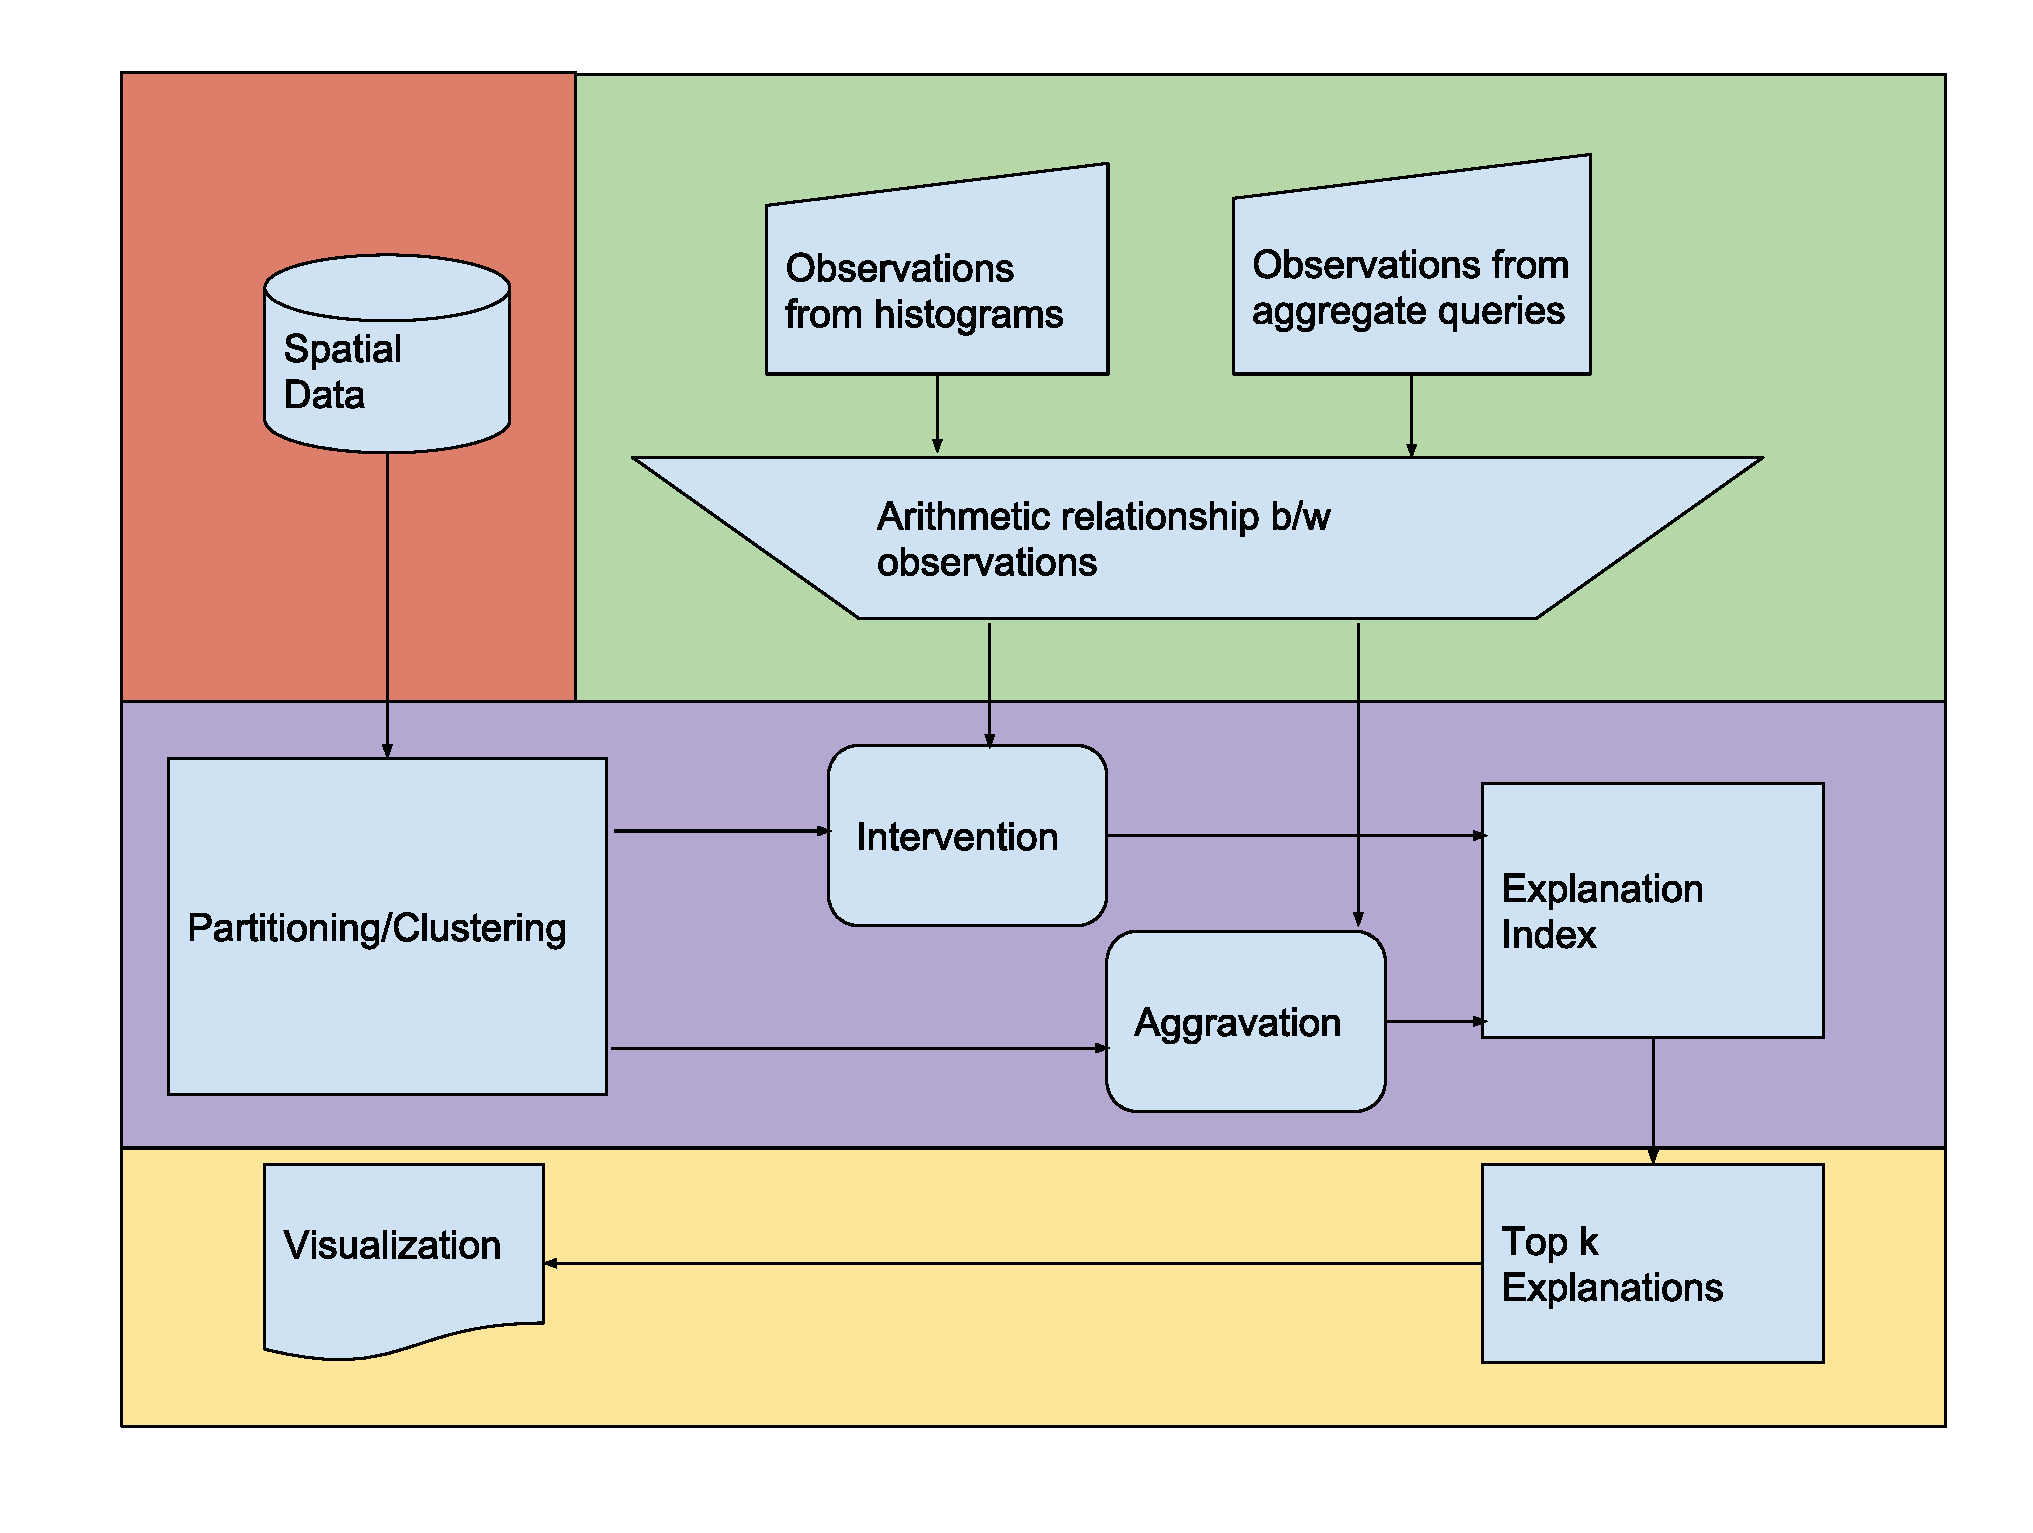
\includegraphics[width=\columnwidth]{framework}
\caption{An outline for our system framework}
\label{fig:framework}
\end{figure}

We created an interface for the system that we have proposed. This interface is web based. It consists of a backend server and a front end for visualizations. The Backend is responsible for querying the Apache Spark daemon with relevant queries. The front end allows the user to define observations and visualize explanations. The front end interface makes use of Mapbox to display the map, Deck.gl to create a visualization overlay on the map. The overlay can be points or polygons. In order to handle state changes in the front end, we used React.js front end library. We also show histograms related to the data. For displaying these histograms, Baidu eCharts library was used. Since the front end was programmed in ES6, webpack was used for transpilation\citep{webpack}. Fig.~\ref{fig:framework} shows us a flow diagram for our system.

In order for the users to easily form observations, our frontend provides them with a series of histograms. Each bar on a histogram represents an aggregate query. Instead of writing queries, the user can easily use the bars in the histograms to be used as variables. These variables can then be used in an arithmetic expression representing the users observations. The user can also define custom variables in the form of aggregate SQL queries manually using the interface.

The back end of the system is an Apache Spark application which calls the Spark daemon for requests of aggravation, intervention, and hierarchical intervention. I must be noted however that there are some operations that the backend performs which are not executed as Spark tasks, such as the creation of an R-Tree. The framework that we have designed requires us to parse and alter queries at multiple points in the pipeline. In order to avoid redesigning the wheel, we use the parser implementation provided by PrestoDB\citep{prestodb}.

To allow the front end to communicate with the backend, there is a middleware application. The job of the middleware is to take the input from the front end and execute our backend application with the appropriate function and input parameters. Our middleware is designed using Node js\citep{tilkov2010node,cantelon2017node}. It takes aggregate queries, selectivity range and number of explanations as input and sends it to the backend application. The results are then sent to the frontend.

\begin{figure}[h]
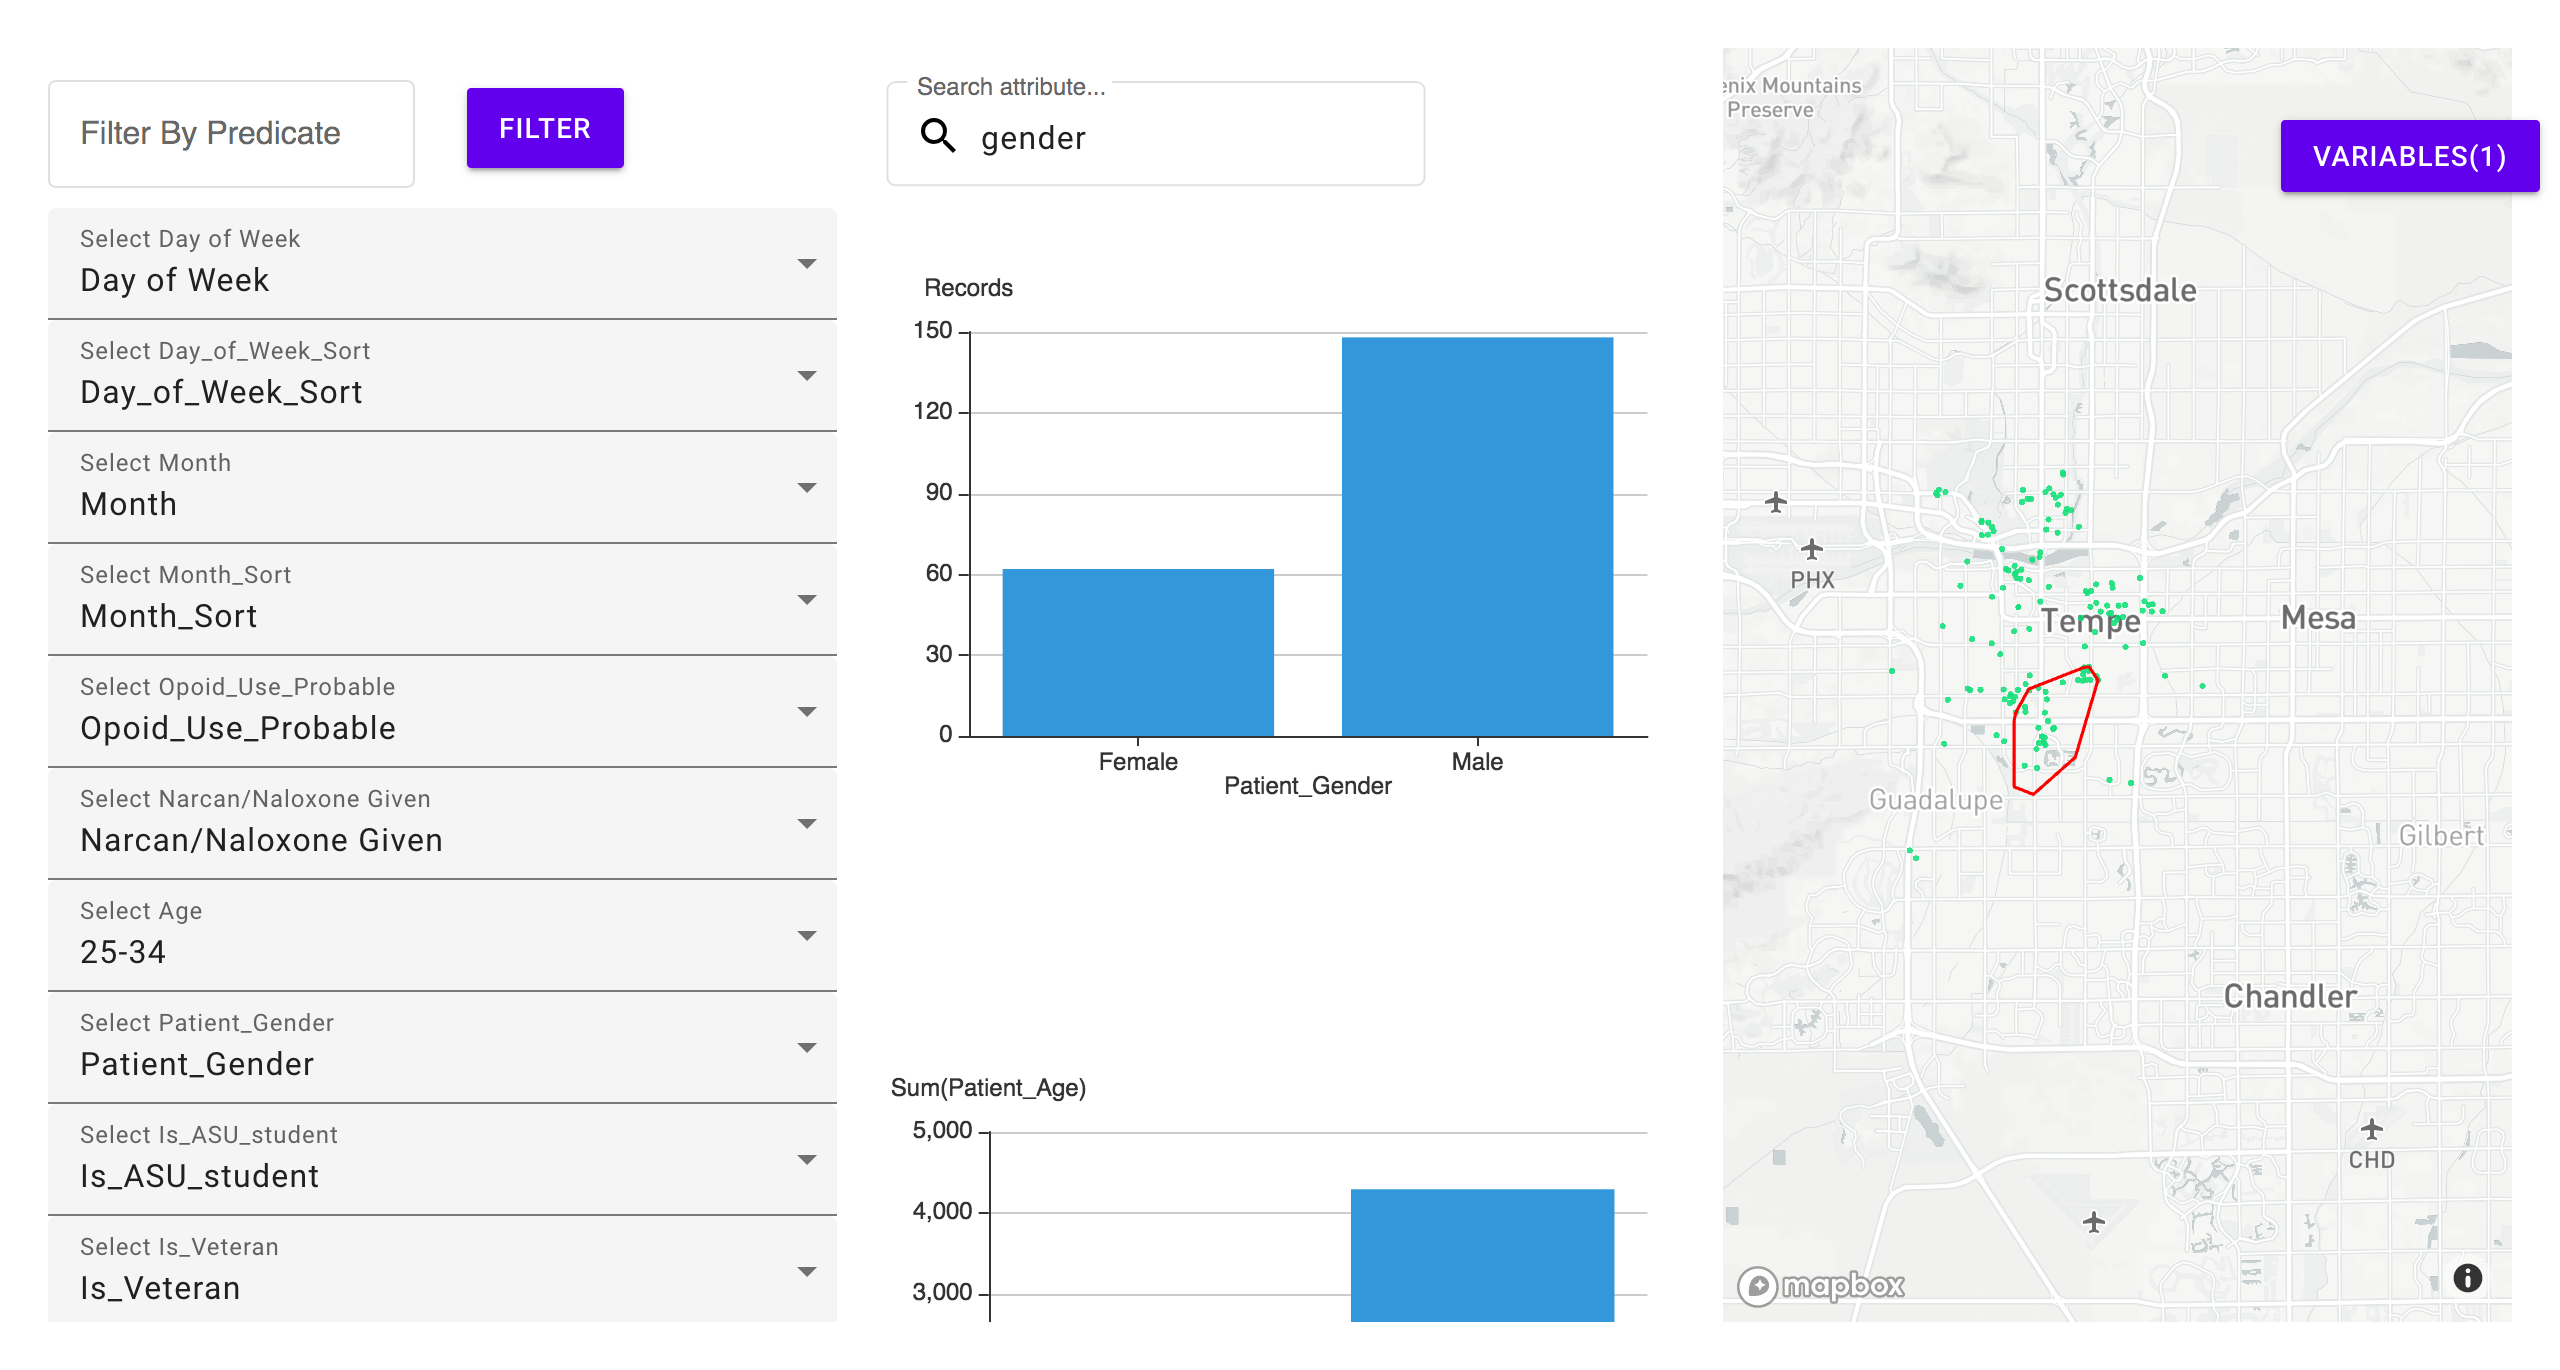
\includegraphics[width=\columnwidth]{interface.png}
\caption{The web interface for our solution}
\label{fig:interface}
\end{figure}

Fig.~\ref{fig:interface} shows the interface that we have created for our solution. The users may add variables from the histograms or they may add them from their own sql queries. The interface allows the user to filter by attribute before viewing the histograms.
